
%% 
%% $Id: intro.tex,v 1.18 2008/03/18 07:14:41 hmj Exp $
%% 
\documentclass[CJKutf8,xcolor=pdftex,dvipsnames,table]{beamer}
\usepackage{hyperref}
\hypersetup{
  pdftitle={Operating System Concepts},
  pdfauthor={Hong MingJian},
  pdfsubject={Introduction},
  pdfpagemode={FullScreen},
  colorlinks={true},
  linkcolor={blue},
}
\usepackage{CJKutf8}
	
\usetheme{Madrid}%{Warsaw}
\usecolortheme{crane}
	
\begin{document}
\begin{CJK*}{UTF8}{song}  

  \title{\CJKfamily{hei} 操作系统原理}
  \subtitle{\CJKfamily{hei} 第一章:介 绍}
	\author{\CJKfamily{hei} 洪明坚}
	\institute{\CJKfamily{hei} 重庆大学软件学院}
  \date{\today}

  \AtBeginSection[]
  {
    \begin{frame}
      \frametitle{Outline}
      \tableofcontents[currentsection]
    \end{frame}
  }

  \frame{\titlepage}

  \frame{\frametitle{目录}\tableofcontents}

  \section{课程简介}
  \subsection{主要内容及参考资料}

  %% PAGE
  \begin{frame}
    \frametitle{课程简介} \pause
	  \begin{itemize}
	    \item{主要内容} \pause
	      \begin{itemize}
	      \item{操作系统的基本概念、原理和设计。} \pause
	      \end{itemize}
	    \item{教材及参考资料} \pause
	      \begin{itemize}
	      \item{\textbf{Abraham Silberschatz, Operating System Concepts, 6th Edition, John Wiley \& Sons, Inc.}} \pause
	        \begin{itemize}
	        \item{9th edition is also available.} \pause
	        \end{itemize}
	      \item{Andrew S. Tanenbaum, Modern operating System, 2nd Edition, Prentice Hall.} \pause
	      \item{Maurice J. Bach, The design of Unix operating system, Pearson education.} \pause
	      \end{itemize}
	    \begin{center}
	    	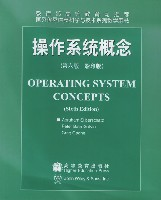
\includegraphics[scale=0.4]{oscv6}  \pause
			\hspace{1mm}
	    	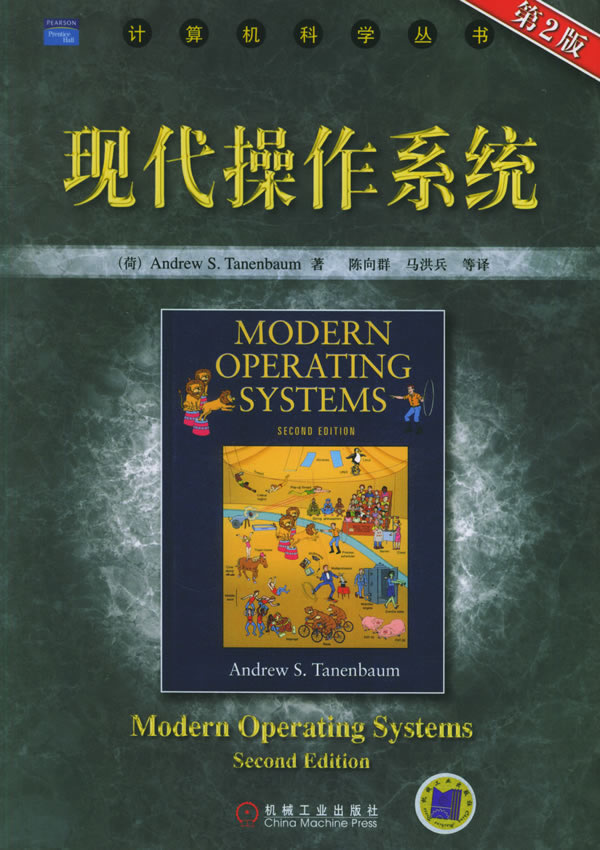
\includegraphics[scale=0.2]{mosv2}  \pause
			\hspace{1mm}
	    	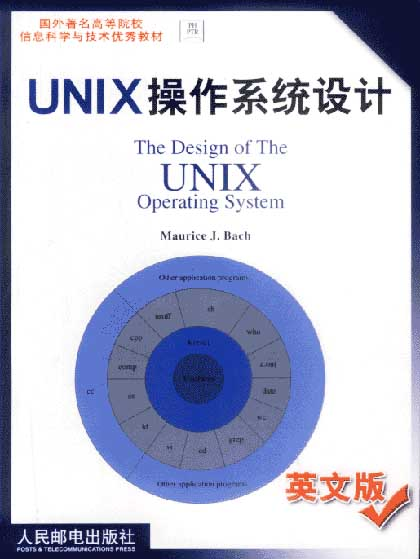
\includegraphics[scale=0.15]{uos}    \pause
	    \end{center}
%	    \item{作业} \pause
%	      \begin{itemize}
%	      \item{记入总成绩,严禁抄袭!}
%	      \end{itemize}
	  \end{itemize}
  \end{frame}

  \subsection{为什么要学习操作系统原理?}

  %% PAGE
  \begin{frame}
    \frametitle{为什么要学习操作系统原理?} \pause
	  \begin{itemize}
	  \item{操作系统是最重要的系统软件之一,} \pause
	    \begin{itemize}
	    \item{没有操作系统的计算机几乎不能使用;} \pause
	    \item{学习操作系统将帮助软件开发人员开发出优秀的应用软件系统。} \pause
	    \end{itemize}
	  \item{操作系统是最复杂的系统软件之一,} \pause
	    \begin{itemize}
	    \item{学习计算机系统是如何工作的;} \pause
	    \item{学习如何通过\textbf{抽象}来掌握复杂的软件系统;} \pause
	    \item{学习如何系统地设计复杂的软件系统。}
	    \end{itemize}
	  \end{itemize}
  \end{frame}

  \section{What's an Operating System?}
  \subsection{Components of a Computer System}

  %% PAGE
  \begin{frame}
    \frametitle{Components of a Computer System} \pause
	  \begin{center}
	    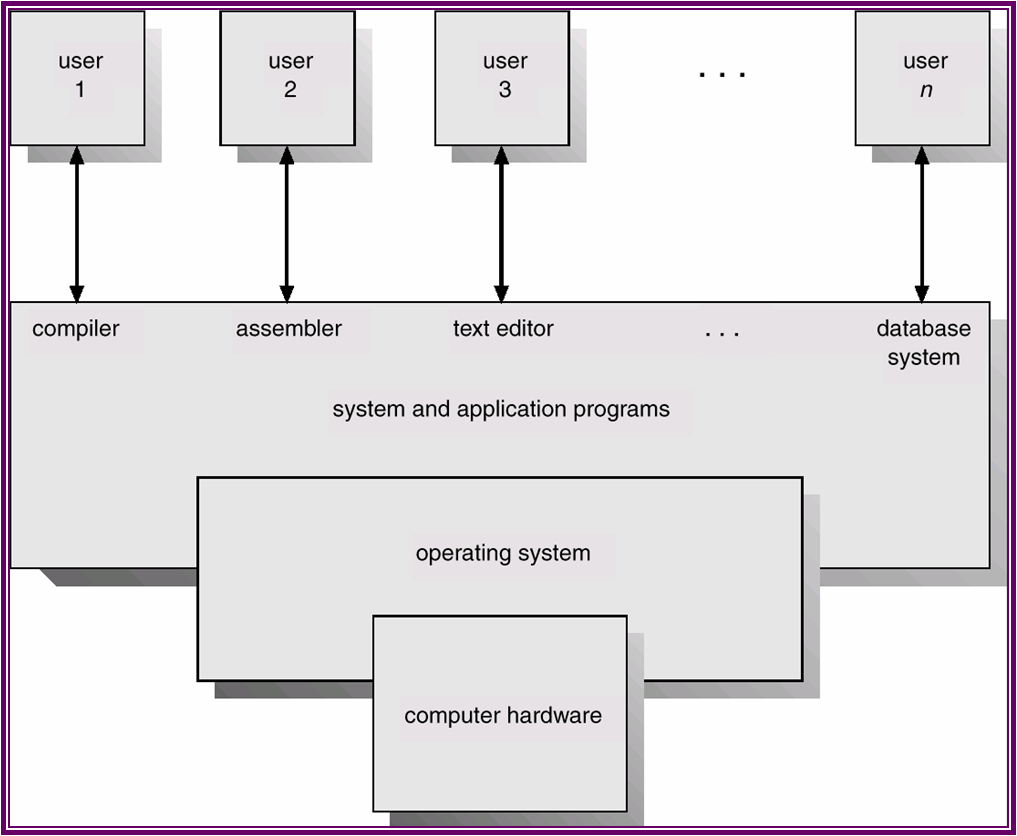
\includegraphics[scale=0.5]{v6f1-1}
	  \end{center}
  \end{frame}

  \subsection{What's an Operating System?}

  %% PAGE
  \begin{frame}
    \frametitle{What's an Operating System?} \pause
	  \begin{itemize}
	  \item{Different views} \pause
	    \begin{itemize}
	    \item{The operating system controls and coordinates the use of the hardware among the various application programs for the various users.} \pause
	      \begin{itemize}
	      \item{\textbf{Control program}} \pause
	      \end{itemize}
	    \item{The operating system manages the resources of a computer so that various applications and users can operate the computer system efficiently and fairly.} \pause
	      \begin{itemize}
	      \item{\textbf{Resource manager (Resource allocator)}} \pause
	      \end{itemize}
	    \item{The operating system abstracts the computer hardware and presents the user a friendly interface.} \pause
	      \begin{itemize}
	      \item{\textbf{Extended machine (Virtual machine)}} \pause
	      \end{itemize}
	    \end{itemize}
	  \item{So, what's an operating system?} \pause
	    \begin{itemize}
	    \item{\textbf{No} common accepted definition is available.} \pause
	    \item{The operating system exists because they are a reasonable way to solve the problem of creating a usable computing system.}
	    \end{itemize}
	  \end{itemize}
  \end{frame}

  \subsection{Components of an operating system}

  %% PAGE
  \begin{frame}
    \frametitle{Components of an operating system} \pause
	  \begin{itemize}
	  \item{What's the part of the operating system?} \pause
	    \begin{itemize}
	    \item{Various people, company or organization has different opinions.} \pause
	      \begin{itemize}
	      \item{Microsoft insists that web browser and media player are parts of the operating system.} \pause
	      \end{itemize}
	    \end{itemize}
	  \item{In this course, we will focus on the \textbf{kernel} of the operating system.} \pause
	    \begin{itemize}
	    \item{The kernel provides the lowest level of abstraction layer for the resources (especially memory, processors and I/O devices). It includes (but is not limited to) the following components} \pause
	      \begin{itemize}
	      \item{\textbf{CPU manager}} \pause
	      \item{\textbf{Memory Manager}} \pause
	      \item{File System} \pause
	      \item{Device Manager}
	      \end{itemize}
	    \end{itemize}
	  \end{itemize}
  \end{frame}

  \subsection{History of Operating System}

  %% PAGE
  \begin{frame}
    \frametitle{History of Operating System} \pause
	  \begin{itemize}
	  \item{To see what operating systems are and what they do, we will consider how they have developed over past 45 years.} \pause
	  \item{Operating system runs on specific hardwares.} \pause
	    \begin{itemize}
	    \item{We cannot understand operating system without some knowledge of underlying hardware.} \pause
	    \end{itemize}
	  \item{So, we will trace the evolution of computer systems and their operating systems to identify the common elements of operating systems.} \pause
	    \begin{itemize}
	    \item{Mainframes and mini-computers} \pause
	      \begin{itemize}
	      \item{Mainframe - IBM System z9} \pause
	      \item{Mini-computer - IBM System i} \pause
	      \end{itemize}
	    \item{Desktop computers} \pause
	      \begin{itemize}
	      \item{Apple II, Macintosh} \pause
	      \item{IBM Personal Computer} \pause
	      \end{itemize}
	    \item{Embedded computers}
	    \end{itemize}
	  \end{itemize}
  \end{frame}

  %% PAGE
  \begin{frame}
    \frametitle{Operating systems for mainframes and minicomputers} \pause
	  \begin{itemize}
	  \item{Mainframes and minicomputers usually have dedicated operating systems.} \pause
	    \begin{itemize}
	    \item{\textbf{zOS} is the operating system for IBM System z9.} \pause
	    \item{\textbf{OS/400} is the operating system for IBM System i.} \pause
	    \end{itemize}
	  \item{They evolved from simple \textbf{batch system}, to \textbf{multiprogramming system} and to \textbf{time-sharing system}.}
	  \end{itemize}
  \end{frame}

  %% PAGE
  \begin{frame}
    \frametitle{Batch systems(1/4)} \pause
	  \begin{itemize}
	  \item{The computer runs one and only one application at a time.} \pause
	  \item{Batching similar jobs} \pause
	    \begin{itemize}
	    \item{Automatically transfers control from one job to another.} \pause
	    \end{itemize}
	  \item{First rudimentary operating system.}
	  \end{itemize}
  \end{frame}

  %% PAGE
  \begin{frame}
    \frametitle{Batch systems(2/4)} \pause
	  \begin{center}
	    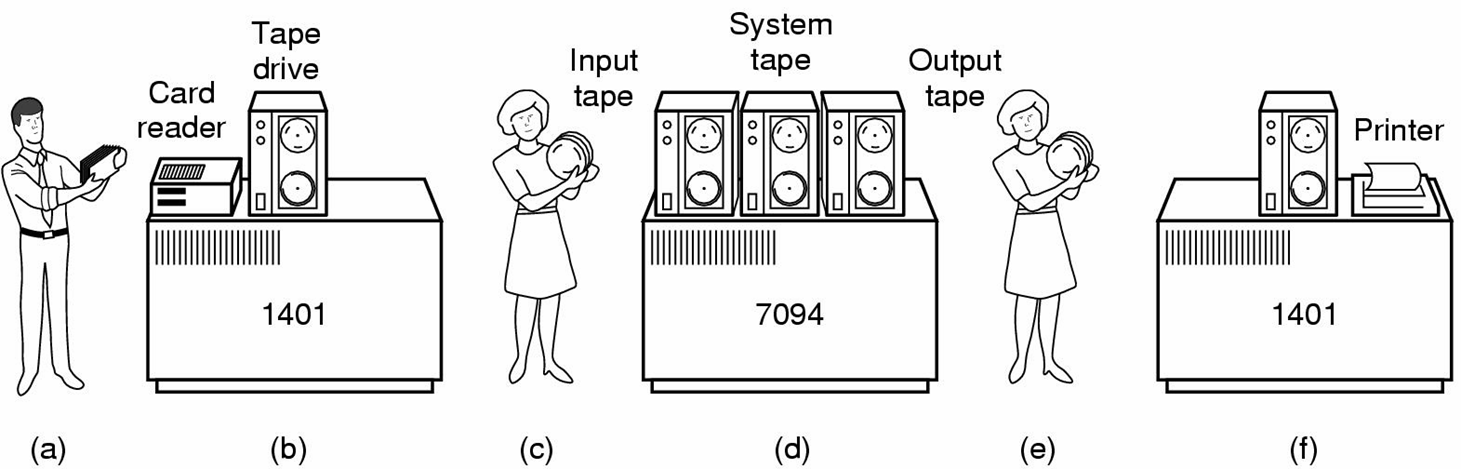
\includegraphics[scale=0.4]{mosv2f1-2} \pause
	  \end{center}
	  \begin{itemize}
	  \item{\scriptsize{(a) Programmers bring cards to IBM 1401} \pause \scriptsize{(b) 1401 reads batch of jobs into tape.}} \pause
	  \item{\scriptsize{(c) Operator carries input tape to IBM 7094} \pause  \scriptsize{(d) 7094 does computing.}} \pause
	  \item{\scriptsize{(e) Operator carries output tape to IBM 1401.} \pause \scriptsize{(f) 1401 prints output.}}
	  \end{itemize}
  \end{frame}

  %% PAGE
  \begin{frame}
    \frametitle{Batch systems(3/4)} \pause
	  \begin{itemize}
	  \item{A typical job: } \pause
	  \end{itemize}
	  \begin{center}
	    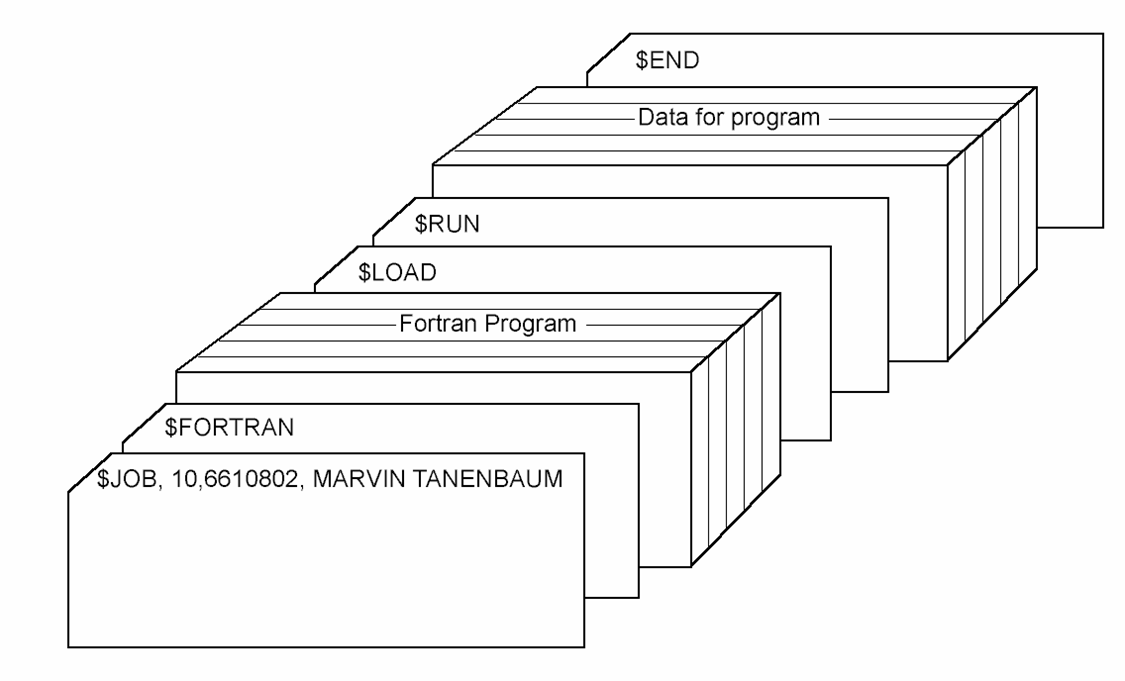
\includegraphics[scale=0.5]{mosv2f1-3}
	  \end{center}
  \end{frame}

  %% PAGE
  \begin{frame}
    \frametitle{Batch system(4/4)} \pause
	  \begin{itemize}
	  \item{A punch card} \pause
	  \end{itemize}
	  \begin{center}
	    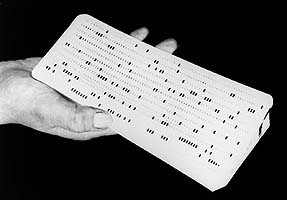
\includegraphics[scale=0.5]{punchcard}
	  \end{center}
  \end{frame}

  %% PAGE
  \begin{frame}
    \frametitle{Multiprogramming systems} \pause
	  \begin{itemize}
	  \item{Several jobs are kept in main memory at the same time, and the CPU is multiplexed among them.} \pause
	  \end{itemize}
	  \begin{center}
	    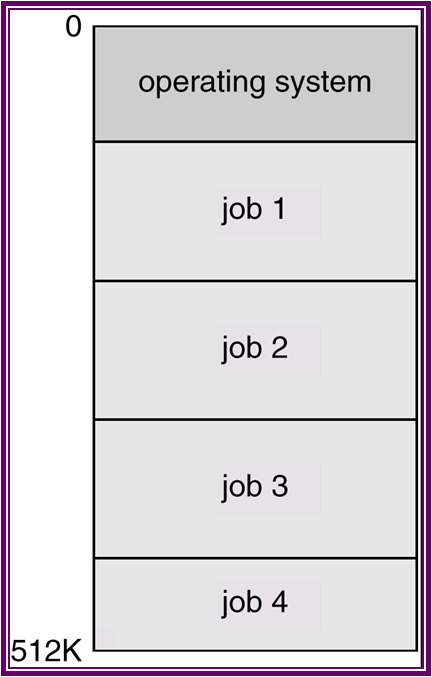
\includegraphics[scale=0.5]{v6f1-3}
	  \end{center}
  \end{frame}

  %% PAGE
  \begin{frame}
    \frametitle{Batch v.s. Multiprogramming system} \pause
	  \begin{center}
	    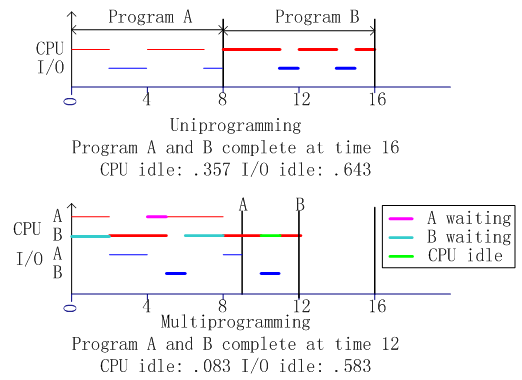
\includegraphics[scale=0.5]{multiprogramming}
	  \end{center}
  \end{frame}

  %% PAGE
  \begin{frame}
    \frametitle{Time-sharing systems} \pause
	  \begin{itemize}
	  \item{The CPU is multiplexed among several jobs that are kept in memory and on disk (the CPU is allocated to a job only if the job is in memory).} \pause
	    \begin{itemize}
	    \item{Designed for interactive computing which requires quick response time.} \pause
	    \end{itemize}
	  \end{itemize}
	  \setlength{\unitlength}{0.5cm}
	  \thicklines
	  \begin{picture}(22, 10)
	    \put(9, 1){\framebox(4, 1.5){CPU}}
	    \put(5, 4){\oval(3, 1.5)}\put(4.3, 3.8){Job 1}
	    \put(8, 6){\oval(3, 1.5)}\put(7.3, 5.8){Job 2}
	    \put(11, 8){\oval(3, 1.5)}\put(10.3, 7.8){Job 3}
	    \put(14, 6){\oval(3, 1.5)}\put(13.3, 5.8){Job 4}
	    \put(17, 4){\oval(3, 1.5)}\put(16.3, 3.8){Job 5}
	    \put(11, 4){\vector(4, 3){2}}
	  \end{picture}
	  \thinlines
  \end{frame}

  %% PAGE
  \begin{frame}
  \frametitle{Operating systems for desktop computers} \pause
	  \begin{itemize}
	  	\item{Operating systems for these computers have benefited in several ways from the development of the operating systems for mainframes.} \pause
	    \begin{itemize}
		    \item{Microsoft MS-DOS, Windows 9x/NT} \pause
		    \item{Apple Macintosh, Mac OS X} \pause
		    \item{IBM OS/2} \pause
		    \item{Unix} \pause
		      \begin{itemize}
		      \item{Solaris by Sun microsystem} \pause
		      \item{HP-UX by Hewlett-Packard} \pause
		      \item{AIX by IBM} \pause
		      \item{Free (as in freedom) software such as \textbf{BSD} (Berkeley Software Distribution) Unix, GNU/Linux} \pause
%		        \begin{itemize}
%		        \item{\textbf{BSD} (Berkeley Software Distribution) Unix, including FreeBSD, OpenBSD and NetBSD} \pause
%		        \item{\textbf{Linux} of GNU (GNU's Not Unix)} \pause
%		        \end{itemize}
		      \end{itemize}
		    \item{......}
	    \end{itemize}
	  \end{itemize}
  \end{frame}

  %% PAGE
  \begin{frame}
    \frametitle{Operating systems for embedded systems} \pause
	  \begin{itemize}
	  \item{Embedded computer is often used as a control device in a dedicated application such as industrial control systems. Usually, they have limited resources: } \pause
	    \begin{itemize}
	    \item{Slow processor, \pause limited memory.} \pause
	    \item{Small or even no display screen.} \pause
	    \item{Limited power supply, etc} \pause
	    \end{itemize}
	  \item{Some control devices have time requirement, i.e., \textbf{Real time}} \pause
	    \begin{itemize}
	    \item{\textbf{Hard real time}, actions absolutely MUST occur at a certain moment.} \pause
	    \item{\textbf{Soft real time}, missing an occasional deadline is acceptable.} \pause
	    \end{itemize}
	  \item{Examples} \pause
	    \begin{itemize}
	    \item{Microsoft Windows CE (Consumer Electronics)} \pause
	    \item{Windriver vxWorks} \pause
	    \item{GNU/Linux, etc}
	    \end{itemize}
	  \end{itemize}
  \end{frame}

  \subsection{Features migration}

  %% PAGE
  \begin{frame}
    \frametitle{Features migration} \pause
	  \begin{itemize}
	  \item{History repeats itself.} \pause
	  \end{itemize}
	  \begin{center}
	    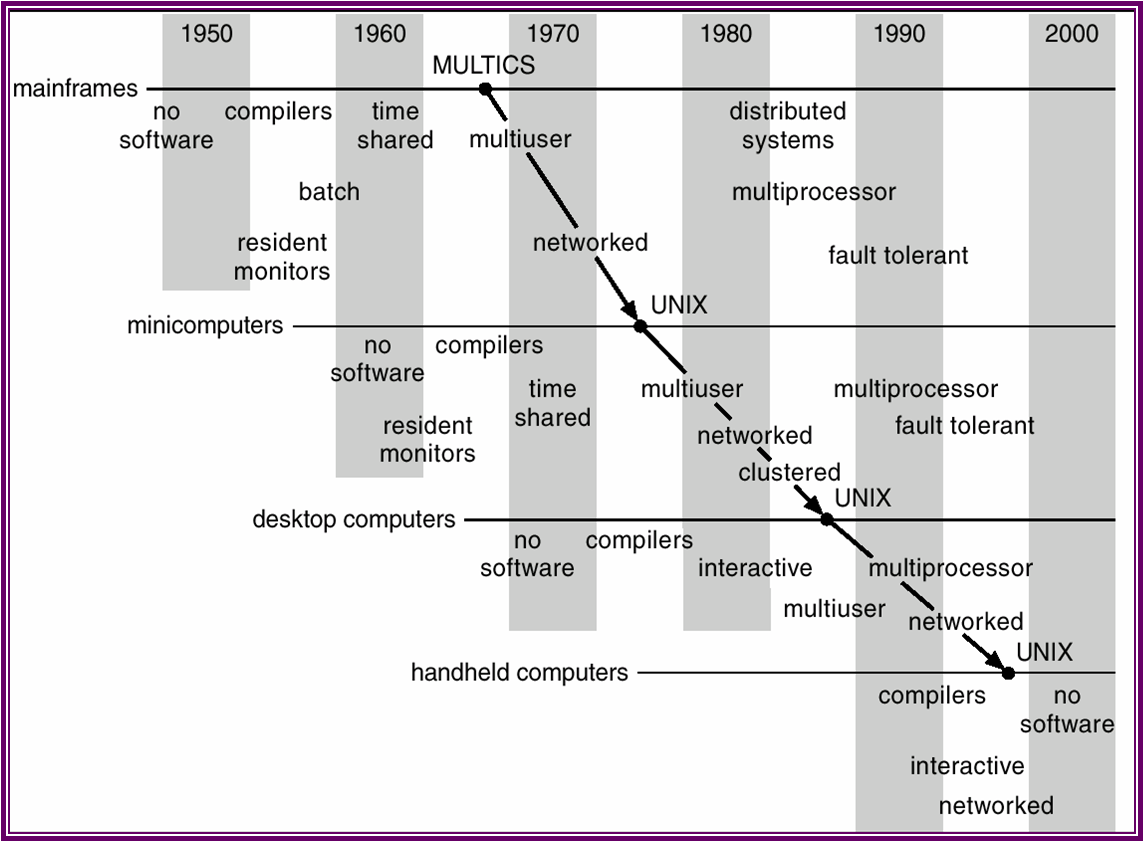
\includegraphics[scale=0.4]{v6f1-6}
	  \end{center}
  \end{frame}

  %% Questions
  \begin{frame}
    \frametitle{Questions}
	  \begin{itemize}
	  \item{Any questions?}
	  \end{itemize}
	  \begin{center}
	    
\includegraphics[scale=.5]{question}
	  \end{center}
  \end{frame}
  
  %% PAGE
\end{CJK*}
\end{document}
